\documentclass{article}


% Packages
\usepackage[utf8]{inputenc} % For Norwegian letters
\usepackage{tabulary} % For nice tables
\usepackage{parskip} % For vertical spacing between paragraphs
\usepackage{float}
\usepackage{graphicx}
\usepackage{caption}
\usepackage{subcaption}
\usepackage{listings}
\usepackage[obeyspaces]{url}

% Config
\setlength{\parindent}{0cm}
\setlength{\parskip}{\baselineskip}

\graphicspath{{images/}}

\begin{document}

% Title
\title{\textbf{Exercise 2} \\ TDT4173}
\author{Simon Borøy-Johnsen \\ MTDT}
\date{\today}
\maketitle
% End Title


% Content
\section{Theory}
\subsection{}
Case based reasoning (CBR) solves problems based on known solutions to similar problems (cases). A case contains a problem, its solution, and usually a description on how the solution was derived. The known problems are compared to the current problem in order to calculate the similarity between them. The solutions for the known cases are then modified in order to fit the problem that is being solved.

The CBR cycle has four main parts:

\begin{enumerate}
    \item Retrieve:

        Given a problem, \textbf{retrieve} similar cases from the memory. These cases should be relevant for solving the problem.
    
    \item Reuse:
    
        The solutions for the known cases are then \textbf{reused} in order to solve the current problem. The solutions are mapped onto the current problem, suggesting how to solve it.
    
    \item Revise:
    
       The suggested solution is then tested (in the real world, or as a simulation). If necessary, the solution is \textbf{revised} to fit the problem even better.
    
    \item Retain:
    
        After a successful solution has been found, the case is \textbf{retained} in memory. By doing this, the case can be used for later problem solving.
\end{enumerate}

The main difference between CBR and other machine learning methods (like rule based ones) lies in when the training examples are generalized. In a rule based algorithm, the training examples are generalized at training time, with no regard to the testing problem. CBR generalized the training examples at testing time. It fetches the relevant known cases according to the problem it is solving.

\subsection{}
Case based reasoning solves problems much in the same way as humans do; it is based on experience, and we adapt known cases onto the problems we try to solve. CBR reasons by remembering. By understanding the cognitive procedures behind our problem solving, we formed the case based reasoning methods.

\subsection{}
Surface similarity is based on high level (surface) features. Usually includes standard value types (strings, symbold, integers, etc.) for measuring similarity. May for example use the "k nearest neighbours" method for determining similarity.

Structural similarity uses domain knowledge, and is highly dependent on the representation of the case. Has the possibility to retrieve cases more relevant to the problem than the similarity measure can.


\section{Practical}
\subsection{Case modelling}
\begin{figure}[H]
  \centering
    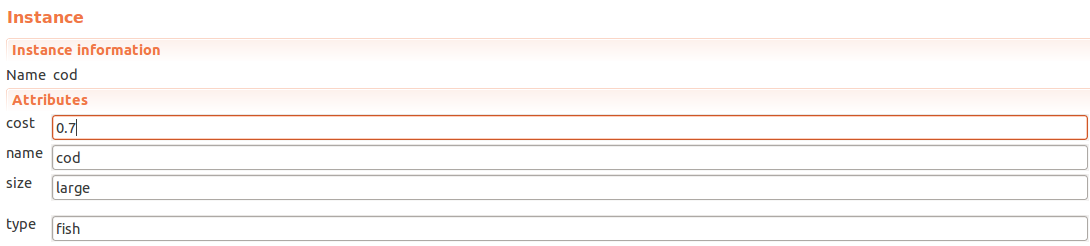
\includegraphics[width=1.0\textwidth]{cod-instance.png}
    \caption{The cod instance}
    \label{fig:cod-instance}
\end{figure}

\subsection{Case retrieval}
\begin{figure}[H]
  \centering
    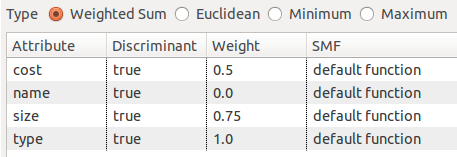
\includegraphics[width=1.0\textwidth]{global-similarity-measure.png}
    \caption{The global similarity measure}
    \label{fig:global-similarity}
\end{figure}

\begin{figure}[H]
  \centering
    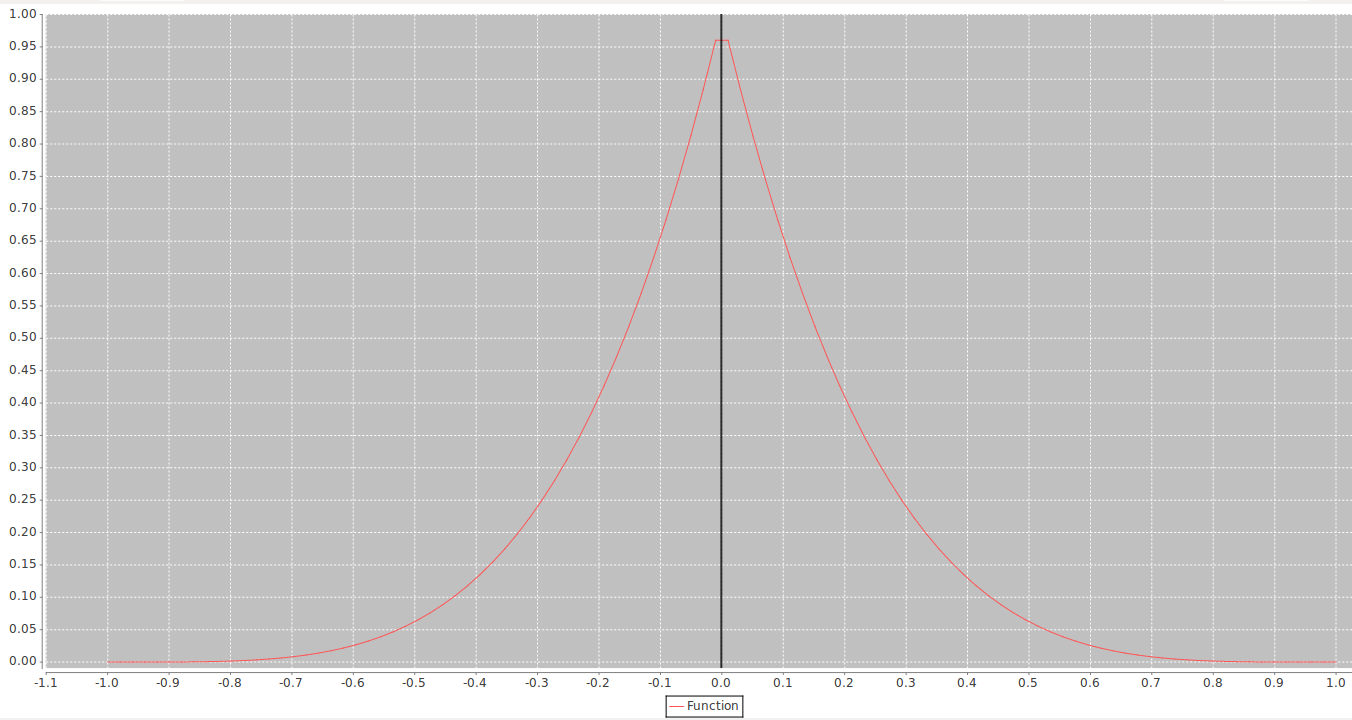
\includegraphics[width=1.0\textwidth]{cost-similarity-measure.png}
    \caption{The default similarity measure for the cost attribute}
    \label{fig:cost-similarity}
\end{figure}

\begin{figure}[H]
  \centering
    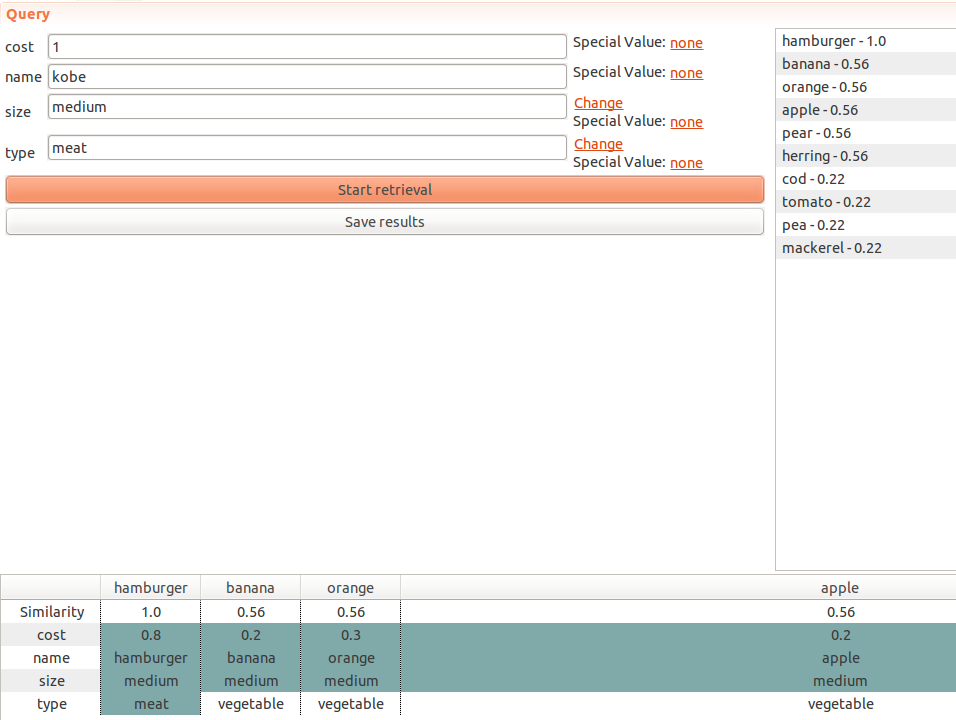
\includegraphics[width=1.0\textwidth]{kobe-search.png}
    \caption{Results when querying Kobe beef}
    \label{fig:kobe-search}
\end{figure}

My most interesting query was the query for Kobe beef. The results can be seen in Figure \ref{fig:kobe-search}.

The hamburger is naturally the clear winner. Both \textit{size} and \textit{type} are exact matches, and the \textit{costs} are almost equal.

I am a bit surprised the banana and orange are second and third, since the \textit{size} is the only match. I would expect the cod to be more similar, but the weight of the \textit{size} outweighs the \textit{type} similarity.

There were no other strange results. Something that can cause strange results is having too few attributes and value spans for the attributes. Take the \textit{size} attribute, for example. How different are the sizes of a hamburger and a beef? It is hard to model exact values for such varying values. Also, so much more can separate a hamburger from a beef. Type of meat, animal, etc.

% End content

\end{document}